\documentclass[12pt,a4paper]{report}

%----------------------------------------------------------------------------------------
%   PACKAGES
%----------------------------------------------------------------------------------------
\usepackage[francais]{babel} %French language package
\usepackage[utf8]{inputenc} %UTF8
\usepackage[T1]{fontenc} %For the acute french accents
\usepackage[pdftex]{graphicx} %To add figures in the document
\usepackage{hyperref} % To make hyperlinks in the document
\usepackage{amsthm} % To add mathematical symbols

\begin{document}
%----------------------------------------------------------------------------------------
%   TITLE PAGE
%----------------------------------------------------------------------------------------
\begin{titlepage}
\newcommand{\HRule}{\rule{\linewidth}{0.5mm}} % Defines a new command for the horizontal lines
\center

%----------------------------------------------------------------------------------------
%   LOGOS SECTION
%----------------------------------------------------------------------------------------

\includegraphics[scale=0.5]{images/umLogo.png} % Université de Montpellier Logo
\hspace{\fill}

\includegraphics[scale=0.25]{images/fdsLogo.jpg} % Faculté de Sciences Logo

%----------------------------------------------------------------------------------------
%   HEADING SECTIONS
%----------------------------------------------------------------------------------------
\textsc{\LARGE M1 Informatique AIGLE}\\[1cm]
\textsc{\Large \textbf{HMIN201}}\\[0.25cm]
\textsc{\large M1 TER}\\[0.5cm]

%----------------------------------------------------------------------------------------
%   TITLE SECTION
%----------------------------------------------------------------------------------------
\HRule \\[0.4cm]
{ \huge \bfseries TER Software Heritage}\\[0.4cm]
{ \Large \bfseries Rapport Final}\\[0.4cm]
\HRule \\[0.5cm]

%----------------------------------------------------------------------------------------
%   AUTHORS AND SUPERVISORS SECTION
%----------------------------------------------------------------------------------------
{ \huge \bfseries Groupe \textsc{Bajonim}}\\[0.4cm]
\begin{minipage}{0.4\textwidth}
\centering \small
\textbf{Bachar \textsc{Rima}}, \\ \href{mailto:bachar.rima@etu.umontpellier.fr}{bachar.rima@etu.umontpellier.fr}\\ % Student
\textbf{Joseph \textsc{Saba}}, \\ \href{mailto:joseph.saba@etu.umontpellier.fr}{joseph.saba@etu.umontpellier.fr}\\ % Student
\textbf{Tasnim \textsc{Shaqura}}, \\ \href{mailto:tasnim.shaqura@etu.umontpellier.fr}{tasnim.shaqura@etu.umontpellier.fr}\\ % Student
\end{minipage} \\[0.8cm]

\begin{minipage}[b]{0.4\textwidth}
\begin{flushleft} \large
\emph{Encadrant:} \\
Jessie \textsc{Carbonnel} % Academic Supervisor
\end{flushleft}
\end{minipage}
~
\begin{minipage}[b]{0.4\textwidth}
\begin{flushright} \large
\emph{Responsable de l'UE:} \\
Mattieu \textsc{Lafourcade} % UE Supervisor
\end{flushright}
\end{minipage}\\[1.5cm]

%----------------------------------------------------------------------------------------
%   DATE SECTION
%----------------------------------------------------------------------------------------
{\large 27 mai 2019}\\[1cm]
\hspace{\fill}
\vfill % Fill the rest of the page with whitespace
\end{titlepage}

%----------------------------------------------------------------------------------------
%   INTRODUCTION
%----------------------------------------------------------------------------------------
\tableofcontents
\chapter{Introduction}
	\section{Description de Software Heritage}
	
	\section{Contexte du TER}
	\section{Plan du rapport}

\chapter{Problématique}
Les logiciels sont actuellement omniprésents dans tous les aspects de notre
vie quotidienne; archiver leurs codes source paraît ainsi une tâche primordiale. À ce titre là, des plateformes ont déjà été proposées, telles que The Internet Archive
et UNESCO Persist. Toutefois, ces plateformes se concentraient plutôt sur la
préservation des fichier exécutables; allant jusqu'à offrir des émulateurs pour permettre l'éxecution des logiciels présents dans leurs archives.
Par comparaison, Software Heritage s'interesse au code source des logiciels, pas à leurs éxecutables. En effet, le code source d'un logiciel constitue un artefact logiciel fondamental dans le domaine des connaisances scientifiques, culturelles, et techniques. Le code source est écrit sous une forme compréhensible par les humains, et peut façilement être transformé en une forme éxecutable par une machine. Le code source est muable et évolue celon les besoins. Ca préservation nous permet d'accéder à l'historique du developement d'un logiciel. 

Malgrés son importance dans notre vie quotidienne, il est façile de voir que nous prennons pas soin correctment du code source. Cela est dû à trois raisons principales.

\section{La diaspora du code source}
Le quantité de projets open sources a vu un énorme accroissement pendant les deux dèrnieres décennies. Le code source de ces projets sont souvent développés sur des plateformes d'hébergement publiques(comme \textit{Github} et \textit{BitBucket}), ou sur des divers forges institutionelles.
Beaucoup d'options s'offrent aux développeurs pour distribuers leurs logiciels. La distribution peut se faire sur des plateforms comme \textit{Github}. Elle peut se faire via des archives liés à des ecosystemes spécifiques, comme \textit{CTAN}, qui distribue des logiciels pour TeX. Les développeurs peuvent aussi choisir de publier leurs logiciels sur des distributions comme \textit{Debian} et \textit{Fedora}, ou via un gestionaire de paquets comme \textit{npm} et \textit{pip}.
\section{La fragilité du code source}
Le code source est une entité fragile. Elle peut être façilement détruite ou perdue si elle n'est pas fréquement sauvegardée. Les plateforms d'hébergement ne guarantient pas forcement la préservation de leurs contenus; des grandes plateformes d'hébergement ont déja arreter leurs services.
\section{Software Heritage en tant que solution}
	Software Heritage a été créer pour relever ces défis. Software Heritage vise a fournir une infrstructure qui permet la collection, l'organisation, le préservation, et l'accés à tout code source publique. L'archive doit avoir la capacité d'accomplir ses objectifs pour toutes plateformes de dévelopement et de distribution, et doit pouvoir persister les codes source sur le long terme.

	\textbf{Current status et roadmap de SWH}
\section{Les défis}
\textbf{Identifier les plateformes d'hébergement :} Les projets peuvent être hébergés sur des plateformes bien connues, comme sur des plateformes obscures. Il faut construire un catalog des plateformes.
\textbf{Supporter differents protocoles : } Software Heritage doit pouvoir recupérer leurs projets et doit pouvoir maintenir les modifications faites sur ces projets. Vu qu les plateformes d'hébergements sont hétérogènes, Software Heritage essayera de promouvoir des bonnes pratiques pour le préservation.
\textbf{Parcourir les historiques de développement :} Les plateformes d'hébergements supportent differents logiciels de gestion de versions qui n'ont pas les même modèles de données. Software Heritage construira un tel modèle unifiant. 
\section{Les principes de base}
\subsection{Transparence et gratuité}
Pour pouvoir assurer la préservation de l'archive sur le long terme, il faut que tout les élements formant l'archive soient open source et accessibles au publique.
\subsection{Réplication compréhensive de l'entiereté du système}
Un tel archive est soumis à differents types de risques. Ces risques étant inévitables, le système doit pouvoir les tolérer. Le système sera répliqué sur differents niveaux: differentes localisations géographiques, differents matériels de stockage , etc...
\subsection{Multitude des partenaires, sans profits}
Pour atteindre ses objectifs, Software Heritage ne doit pas dépendre sur une seule entité qui cherche d'en profiter, et ne doit pas être créer pour la géneration de profits. Ce projet doit apporter de la valeur au public en large, et non seulement pour les organisations qui le supporte.
\subsection{Pas de présélection}
 Il est impossible de savoir quel projets vont finir par être les plus importants. Il faut doc préserver tout les logiciels disponibles sans présélection, surtout que la capacité technique de faire cela est disponible. 
\subsection{Source Code First}
Bien qu'il est intéressant de garder le contexte du code source (comme les Wiki, l'environement où le programme est éxécuté, etc), une telle tâche nécessite une énorme quantité de resources, surtout qu'il n'y a pas de préselection. Software Heritage se contente d'archiver les code sources ainsi que leur historique de développement capturé par les logiciels de gestion de versions. Cela permet de guarder des informations importantes qu'on retrouve dans les messages de commit.
\subsection{Identifiants Intrinsèque}
Les identifiants des objets stockés ne doivent pas dépendre des sources externes et doivent pouvoir être calculés à partir des objets qu'ils identifient. Ils sont étroitement liés à ces objets. Cela permet de verifier que l'objet obtenu correspond à l'objet demandé, et permet la détection les modifications sur l'objet.
\subsection{Informations de provenance et informations factuelles}
Software Heritage va stocké les informations de provenance qui décrivent le ou, le quoi, et le quand des objets dans l'archive. Ces informations vont être verifiés et les méthodes de verification vont être stockées aussi.
\subsection{Minimalisme}
Software Heritage se contentera de construire l'infrastructure essentielle et rien de plus.
\section{Notre travail}
Dans le cadre de ce projet, encadré par Jessie Carbonnel, nous avons cibler la plateforme d'hébergement Launchpad afin de collectioner les codes sources qui y sont hébergés, et les stocker dans l'archive de Software Heritage. Ainsi, les objectifs de ce TER peuvent être énumérés de la manière suivante :
\begin{itemize}
\item Lire/comprendre les articles et tutoriels écrits par l'équipe de Software Heritage;
\item Analyser différentes plateformes d'hébergement afin d'en cibler une;
\item Concevoir et développer un Lister pour la plateforme choisie;
\item Répliquer localement l'environnement de Software Heritage afin de tester le Lister développé;
\item Faire une Pull Request afin d'intégrer le Lister testé au dépôt de développement de Software Heritage.
\end{itemize}

\chapter{Analyse}
\section{Fonctionnement de Software Heritage}
	\subsection{Modèle des données}
		\subsubsection{Plateformes d'hébergement}
		\subsubsection{Artéfacts logiciels}
		\subsubsection{Informations sur la provenance des données}
		\subsubsection{Structure des données}
	\subsection{Architecture et flot des données}
		\subsubsection{Flot d'ingestion des données}
		\subsubsection{Listing}
		\subsubsection{Loading}
		\subsubsection{Scheduling}
	\subsection{L'archive}
		\subsubsection{Stockage des noeuds BLOB de l'archive}
				les IDs, les fichiers
		\subsubsection{Stockage des autres noeuds des archives}
				chemins, repertoires, snapshot, revisions, releases\\				
				postgres, etc
		\subsubsection{Stockage haché des objets}
		\subsubsection{Mise en mirroir des noeuds}
		\subsubsection{Politique de rétention}
		\subsubsection{Récupération automatique des objects corrompus}
\section{Méthodologie}		
	Sourceforge sitemap, api\\
	Launchpad api, client\\
	Analyzing the listers (bitbucket, gitlab, github, eclipse, LIRMM, OpenHub, 			Assembla, GNU savannah\\
	heritage, injection de dependances\\
	conclusion: on adoptera une strategie pour definir un lister, loader ou autre\\
\section{Planning Prévisionnel}
\chapter{Conception}
	design de la solution proposée (diagrammes + explications)
\chapter{Implémentation}
	Les Listers de Software Heritage et les codes qui les accompagnent sont écrits en Python. 
	
	\section{Le client Launchpad}
	les technos qu'on a utilisé\\
	bibliotheques\\
	Outils (e.g. XML parsers)\\
	parler du client
	parler du notebook
	parler du code qu'on a créer par rapport au client (les classes du proxy)
	parler du JSON et de son format, et comment il est mapped to SWH's model
		
\chapter{Résultats}
	pull request?
\chapter{Conclusion}
	\section{Planning final}
	\begin{figure}[!ht]
	\hspace*{-3cm}
	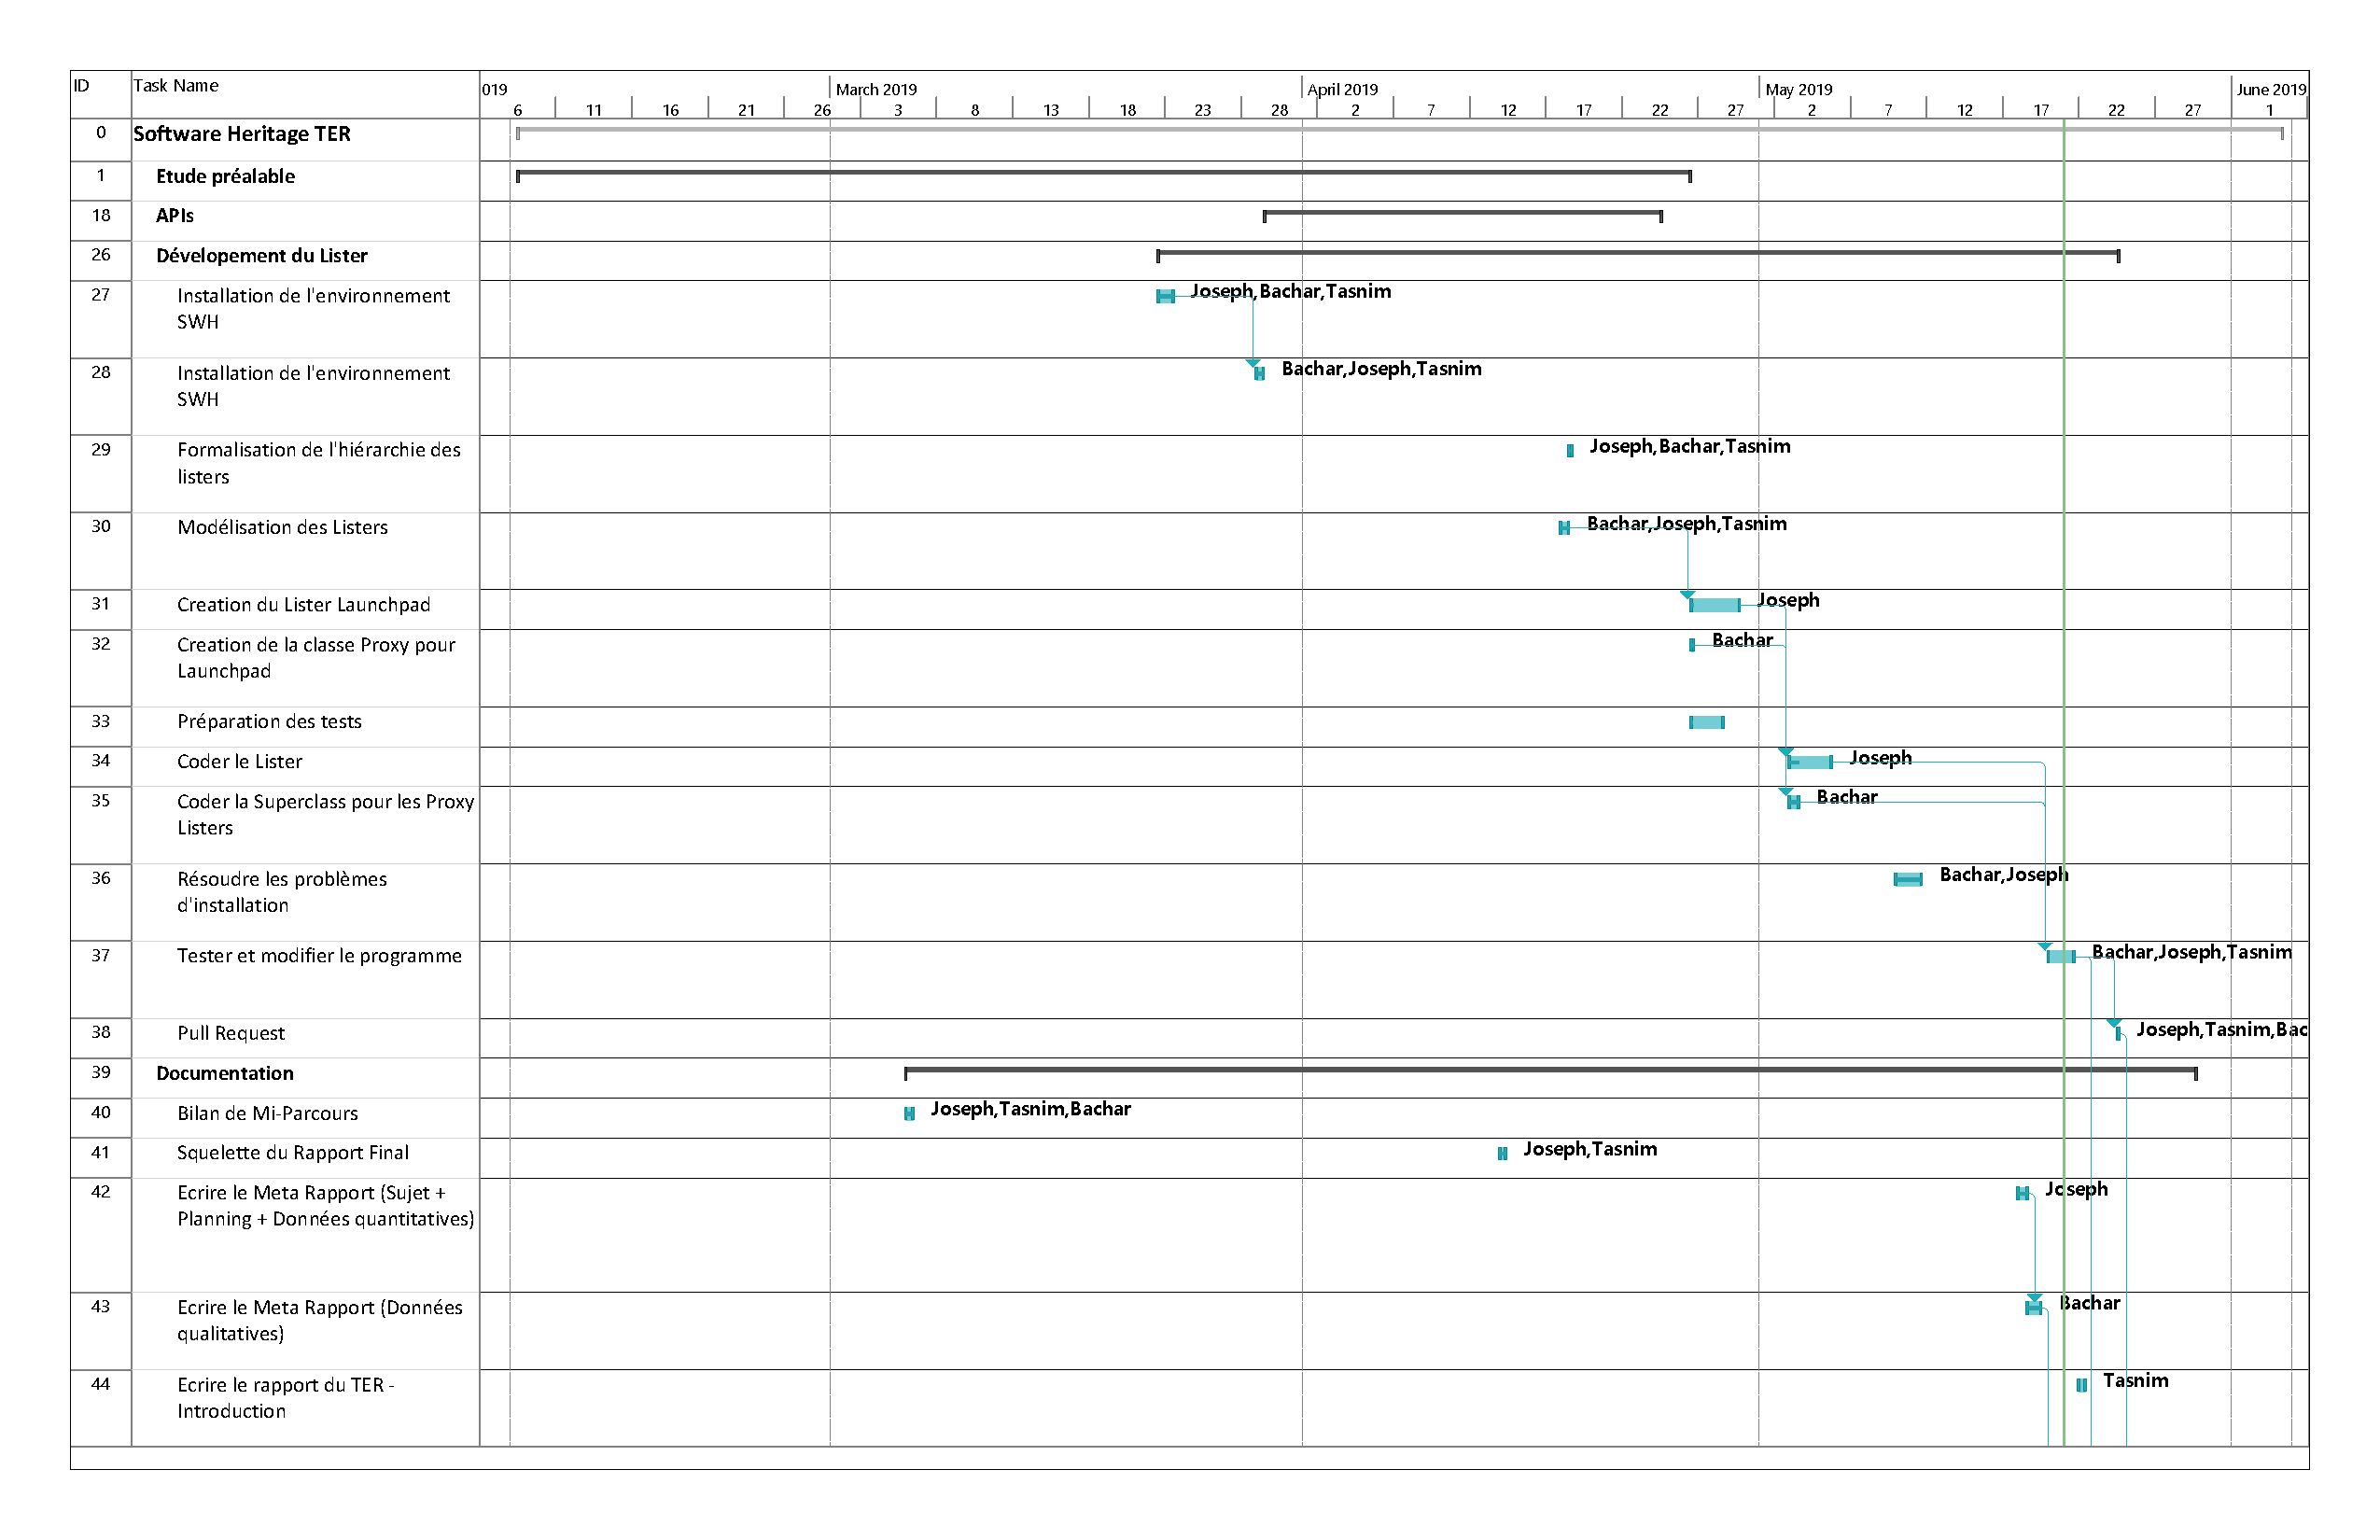
\includegraphics[scale=0.45]{pdfs/planning_final_summary.pdf}
	\end{figure}
	\begin{figure}[!ht]
	\hspace*{-3cm}
	\includegraphics[scale=0.45,page=2]{pdfs/planning_final_summary.pdf}
	\caption{Planning final}
	\end{figure}

	\section{Difficultés rencontrées}
	Au cours de se projet, nous avons rencontrer des difficultés auxquelles nous ne nous attendions pas.
	\subsection{Les APIs}
	\subsection{Les tests}
	
	\section{Perspectives}
	ce qu'on a fait (extensibilité du code, le fait qu'il est parametrable grace au classes abstraites)
	ce qu'on peut améliorer (les tests? informations du context)
	\section{Bilan et apports du TER}	
annexes
\t resumés \t code	
\chapter*{Bibliographie}
%todo%
1)Software Heritage: Why and How to Preserve Software Source Code - Roberto Di Cosmo, Stefano Zacchiroli
2) Identifiers for Digital Objects: the Case of Software Source Code Preservation - Roberto Di Cosmo, Morane Gruenpeter, Stefano Zacchirol
\end{document}